\begin{frame}{Distributions of Random Variables}
    \begin{itemize}
        \item We've spent the past week talking about random variables.
        \item We've also talked about probability distributions.
    \end{itemize}
    \vspace{12pt}In Chapter 4, we are going to put these two concepts together to think about some common distributions that we use to model random variables.
\end{frame}

\begin{frame}{The Normal Distribution}
    We start our discussion with the \textbf{normal distribution}. This is one of the most common distributions you will see in practice.
    
    \begin{center}
        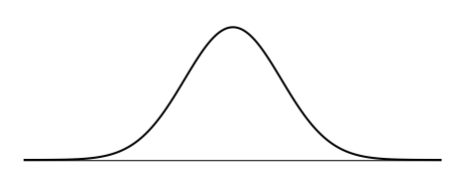
\includegraphics[scale=0.5]{images/normalcurve.png}
    \end{center}
\end{frame}

\begin{frame}{The Normal Distribution}
    \begin{center}
        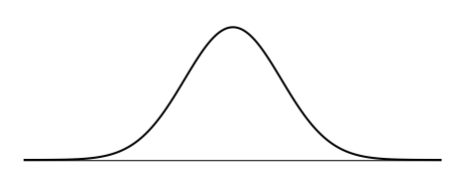
\includegraphics[scale=0.5]{images/normalcurve.png}
    \end{center}
    
    Normal distributions are always...
    \begin{itemize}
        \item Symmetric.
        \item Unimodal.
        \item "Bell curves".
    \end{itemize}

    Variables such as SAT scores closely follow the normal distribution.
\end{frame}

\begin{frame}{The Normal Distribution}
    \begin{center}
        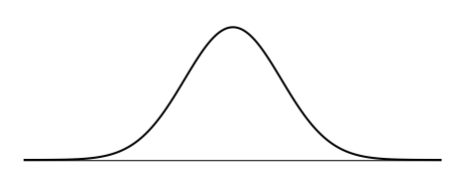
\includegraphics[scale=0.5]{images/normalcurve.png}
    \end{center}
    
    The normal distribution has most measurements falling somewhere near the middle - or average - and values get less and less likely as we move further into the tails.
    
    \vspace{12pt}Variables such as SAT scores closely follow the normal distribution.
\end{frame}

\begin{frame}{Normal Distributions}
    \begin{itemize}
        \item Many variables are nearly normal, but none are exactly normal. 
        \item While not perfect for any single problem, the normal distribution is very \textit{useful} for a variety of problems. 
        \item We will use it in data exploration and to solve important problems in statistics.
    \end{itemize}
\end{frame}

\begin{frame}{The Normal Distribution Model}
    \begin{itemize}
        \item The symmetric, unimodal, bell-shaped curve of the normal distribution can vary based on:
        \begin{itemize}
            \item Mean
            \item Standard deviation
        \end{itemize}
        \item These adjustable details are called \textbf{model parameters}.
    \end{itemize}
\end{frame}

\begin{frame}{Parameters: Normal Distribution}
    \begin{center}
        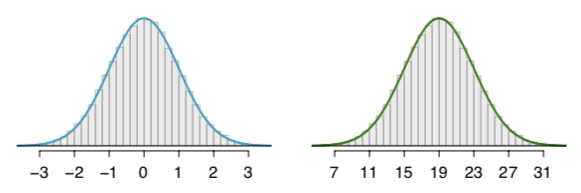
\includegraphics[scale=0.5]{images/meansd_normal.png}
    \end{center}
    \begin{itemize}
        \item Changing the mean shifts the curve to the left or right.
        \item Changing the standard deviation stretches or constricts the curve.
        \begin{itemize}
            \item (This can make the peak appear narrower or flatter.)
        \end{itemize}
    \end{itemize}
\end{frame}

\begin{frame}{Parameters: Normal Distribution}
    \begin{center}
        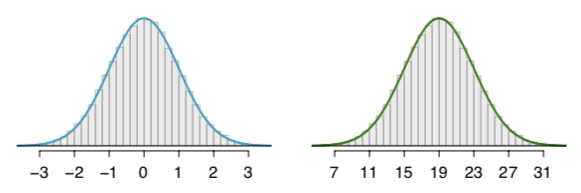
\includegraphics[scale=0.5]{images/meansd_normal.png}
    \end{center}
    \begin{itemize}
        \item The distribution on the left has $\mu=0$ and $\sigma=1$.
        \item The distribution on the right has $\mu=19$ and $\sigma=4$
        \item These look exactly the same because the scale of the axis has been adjusted. 
    \end{itemize}
\end{frame}

\begin{frame}{Parameters: Normal Distribution}
    \begin{center}
        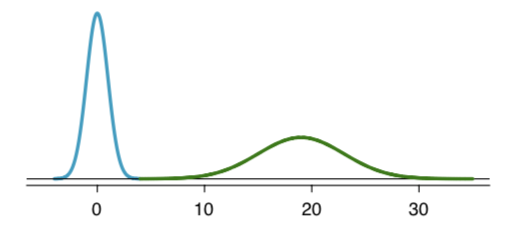
\includegraphics[scale=0.5]{images/meansd_nrml.png}
    \end{center}
    \vspace{-12pt}\begin{itemize}
        \item These are the same two distributions, now on the same axis.
        \item Now we can see that the shift of the mean from $0$ to $19$ moves the distribution to the right.
        \item The change in standard deviation from $1$ to $4$ flattens the distribution.
    \end{itemize}
\end{frame}

\begin{frame}{Normal Distribution Notation}
    For a normal distribution with mean $\mu$ and standard deviation $\sigma$, we write
    \[
        N(\mu, \sigma)
    \]
    For a variable $X$ with a normal distribution, we may write
    \[
        X \sim N(\mu, \sigma).
    \]
    where "$\sim$" denotes "is distributed".
\end{frame}

\begin{frame}{Normal Distribution Notation}
    For a normal distribution with mean $19$ and standard deviation $4$, we write
    \[
        N(\mu=19, \sigma=4)
    \]
    \begin{itemize}
        \item The mean and standard deviation describe a normal distribution fully and exactly. 
        \item This is what we mean by a distribution's \textbf{parameters}.
    \end{itemize}
\end{frame}

\begin{frame}{Standard Normal Distribution}
    The \textbf{standard normal distribution} is a normal distribution with mean $\mu=0$ and standard deviation $\sigma=1$.
    \[
        N(\mu=0, \sigma=1)
    \]
\end{frame}

\begin{frame}{Standardizing with Z-Scores}
    We often want to put data onto a standardized scale, which can make comparisons more reasonable.
\end{frame}

\begin{frame}{Example: SAT and ACT}
    The distribution of SAT and ACT scores are both nearly normal. The table shows the mean and standard deviation for total scores on each. 
    \begin{center}
        \begin{tabular}{l cc}
            \hline
            & SAT & ACT  \\
            \hline
            Mean & 1100 & 21 \\
            SD & 200 & 6 \\
            \hline
        \end{tabular}
    \end{center}
    Suppose Ann scored 1300 on her SAT and Tom scored 24 on his ACT. Who performed better?
\end{frame}

\begin{frame}{Example: SAT and ACT}
    \begin{itemize}
        \item We can use the standard deviation to help us figure out who performed better.
        \item Ann's SAT score is 1 standard deviation above average.
        \begin{itemize}
            \item $1100 + 200 = 1300$
        \end{itemize}
        \item Tom's ACT score is 0.5 standard deviations above average.
        \begin{itemize}
            \item $21 + 0.5 \times 6 = 24$
        \end{itemize}
        \item If you remember taking either test and being told your percentile, that's the same idea!
    \end{itemize}
\end{frame}

\begin{frame}{Example: SAT and ACT}
    We can also plot the normal distributions with scaled axes:
    \begin{center}
        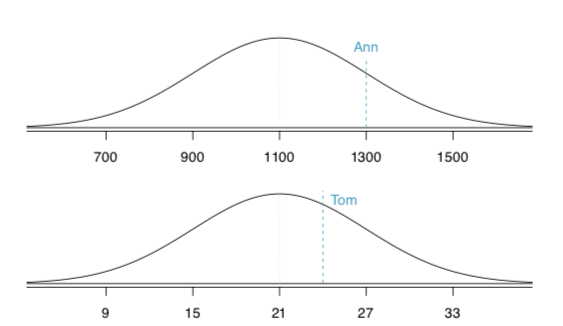
\includegraphics[scale=0.4]{images/actsat.png}
    \end{center}
    Now we can see that Ann tends to do better with respect to everyone else than Tom does, so her score is better.
\end{frame}

\begin{frame}{Standardizing with Z-Scores}
    Our example got at a standardization technique called a Z-score.
    \begin{itemize}
        \item This method is commonly employed with normal distributions, but could also be used more generally.
        \item The \textbf{Z-score} of an observation is defined as the number of standard deviations it falls above or below the mean.
        \begin{itemize}
            \item If the observation is one standard deviation above the mean, its Z-score is 1.
            \item If it is 1.5 standard deviations below the mean, then its Z-score is -1.5.
        \end{itemize}
    \end{itemize}
\end{frame}

\begin{frame}{Standardizing with Z-Scores}
    We compute the Z-score for an observation $x$ that follows a distribution with mean $\mu$ and standard deviation $\sigma$ using
    \[
        z = \frac{x-\mu}{\sigma}
    \]
\end{frame}

\begin{frame}{Example: Standardizing with Z-Scores}
    The SATs had a mean score of $\mu_{SAT}=1100$ and a standard deviation of $\sigma_{SAT}=200$. For Ann's SAT score of 1300, the Z-score is
    \[
        z_{Ann}=\frac{x_{Ann}-\mu_{SAT}}{\sigma_{SAT}} = \frac{1300-1100}{200} = 1
    \]
\end{frame}

\begin{frame}{Example: Standardizing with Z-Scores}
    The ACTs has mean $\mu=21$ and standard deviation $\sigma=6$. Use Tom’s ACT score, 24, to find his Z-score.
\end{frame}

\begin{frame}{Z-Scores}
    \begin{itemize}
        \item Observations above the mean always have positive Z-scores.
        \item Observations below the mean always have negative Z-scores. 
        \item If an observation is equal to the mean, the Z-score is always 0.
    \end{itemize}
\end{frame}

\begin{frame}{Example}
    Let $X$ represent a random variable from $N (\mu = 3, \sigma = 2)$
    \[
        X \sim N (\mu = 3, \sigma = 2)
    \]
    and suppose we observe $x = 5.19$.
    \begin{enumerate}
        \item Find the Z-score of x.
        \item Use the Z-score to determine how many standard deviations above or below the mean x falls.
    \end{enumerate}
\end{frame}

\begin{frame}{Example}
    We know from the problem statement that $\mu = 3$, $\sigma = 2$, and our observed value is $x=5.19$. So
    \begin{align*}
        z &= \frac{x-\mu}{\sigma} \\
            &= \frac{5.19-3}{2} \\
            &= 1.095.
    \end{align*}
\end{frame}

\begin{frame}{Example}
    Using our definition of a Z-score, $z = 1.095$ means that the observations $x$ is $1.095$ standard deviations \textit{above} the mean.
    
    \vspace{12pt}We know that $x$ is above the mean because the Z-score is positive.
\end{frame}

\begin{frame}{Example: Brushtail Possums}
    Head lengths of brushtail possums follow a normal distribution with mean 92.6 mm and standard deviation 3.6 mm. 
    
    \vspace{12pt}Compute the Z-scores for possums with head lengths of 95.4 mm and 85.8 mm.
\end{frame}

\begin{frame}{Example: Brushtail Possums}
    Let $Y$ be the head lengths of brushtail possums. We say that $Y\sim N(\mu=92.6, \sigma=3.6)$.
    
    \vspace{12pt}For a head length of 95.4 mm, the Z-score will be
    \begin{align*}
        z &= \frac{y-\mu}{\sigma} \\
            &= \frac{95.4-92.6}{3.6} \\
            &= 0.78.
    \end{align*}
\end{frame}

\begin{frame}{Example: Brushtail Possums}
    Let $Y$ be the head lengths of brushtail possums. We say that $Y\sim N(\mu=92.6, \sigma=3.6)$.
    
    \vspace{12pt}For a head length of 85.8 mm, the Z-score will be
    \begin{align*}
        z &= \frac{y-\mu}{\sigma} \\
            &= \frac{85.8-92.6}{3.6} \\
            &= -1.89.
    \end{align*}
\end{frame}

\begin{frame}{Example: Brushtail Possums}
    \begin{center}
        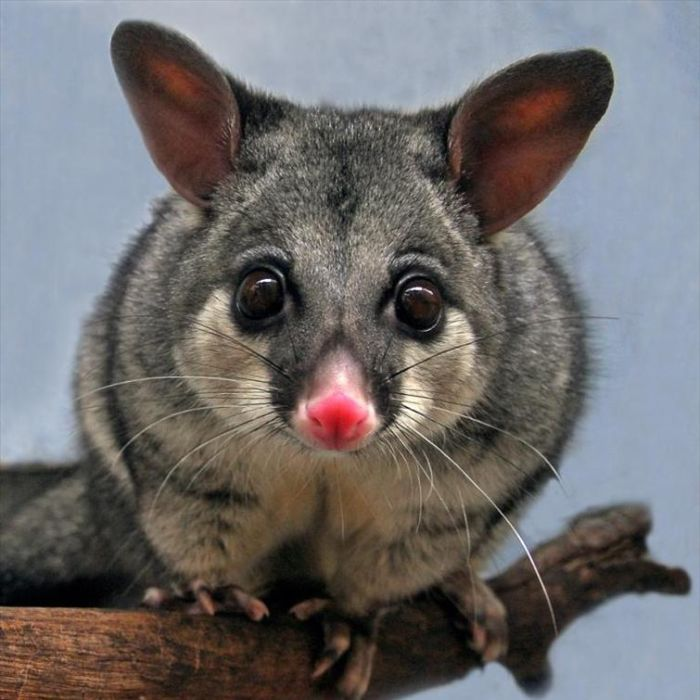
\includegraphics[scale=0.2]{images/possum.jpg}
    \end{center}
    \vspace{-12pt}\begin{itemize}
        \item The possum with a head length of 95.4 mm is 0.78 standard deviations \textit{above} the mean ($z=0.78$).
        \item The possum with a head length of 85.8 mm is 1.89 standard deviations \textit{below} the mean ($z=-1.89$).
    \end{itemize}
\end{frame}

\begin{frame}{Z-Scores and Unusual Observations}
    \begin{itemize}
        \item We can use Z-scores to identify potentially unusual observations.
        \item An observation $x_1$ is \textit{more unusual} than another observation $x_2$ is further from the mean.
        \item If $z_1$ and $z_2$ are the corresponding Z-scores, $x_1$ is more unusual than $x_2$ if
        \[
            |z_1| > |z_2|
        \]
        \item This technique is especially useful for symmetric distributions.
    \end{itemize}
\end{frame}

\begin{frame}{Example: Brushtail Possums}
    We decided that
    \begin{itemize}
        \item The possum with a head length of 95.4 mm is 0.78 standard deviations \textit{above} the mean ($z=0.78$).
        \item The possum with a head length of 85.8 mm is 1.89 standard deviations \textit{below} the mean ($z=-1.89$).
    \end{itemize}
    Since 
    \[
        |-1.89| > |0.78|,
    \]
    we say the possum with the head length of 85.8 mm is more unusual than the other possum.
\end{frame}

\begin{frame}{Finding Tail Areas}
    \begin{itemize}
        \item Yesterday, we talked about using the area under a curve to think about proportions.
        \item Determining the area under the tail of a distribution is very useful in statistics!
        \item For example, your SAT percentile is the fraction of people who scored lower than you.
    \end{itemize}
\end{frame}

\begin{frame}{Finding Tail Areas}
    We can visualize a tail area as the curve and shading shown. 
    \begin{center}
        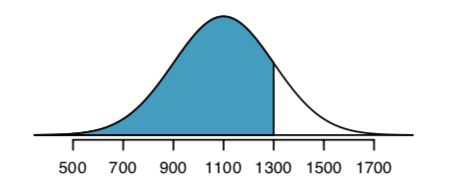
\includegraphics[scale=0.5]{images/tailarea.png}
    \end{center}
    \begin{itemize}
        \item This is the distribution for SAT scores with Ann's score as the cutoff point, at $x=1300$.
        \item The area to the left of $x$ is the percentile.
    \end{itemize}
\end{frame}

\begin{frame}{Finding Tail Areas}
    There are several techniques for finding tail areas:
    \begin{enumerate}
        \item Integrate.
        \item Use a graphing calculator.
        \item Use a probability table.
        \item Use a statistical software.
    \end{enumerate}
\end{frame}

\begin{frame}{Finding Tail Areas: Integration}
    The function that creates our normal distribution curve is
    \[
        f(x) = \frac{1}{\sqrt{2\pi\sigma^2}}e^{-\frac{(x-\mu)^2}{2\sigma^2}}
    \]
    Don't write this down. We won't use it. In fact, it's impossible to integrate this by hand!
\end{frame}

\begin{frame}{Finding Tail Areas: Graphing Calculator}
    You are not required to have a graphing calculator, so you won't be required to use one for tail probabilities.
    
    \vspace{12pt}However, you can find a video of how to use a graphing calculator to calculate tail probabilities at 
    \begin{center}
        www.openintro.org/videos
    \end{center}
\end{frame}

\begin{frame}{Finding Tail Areas: Probability Tables}
    Probability tables are often used in classrooms but these days they are rarely used in practice. 
    
    \vspace{12pt}Appendix C.1 in your textbook contains such a table and a guide for how to use it.
\end{frame}

\begin{frame}{Finding Tail Areas: Software}
    Since we can't integrate by hand, we can have a computer integrate for us!
    \begin{center}
        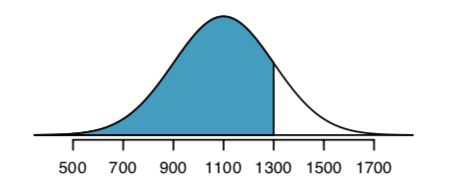
\includegraphics[scale=0.5]{images/tailarea.png}
    \end{center}
    In \texttt{R}, we could find the area shown using the following command, which takes in the Z-score and returns the lower tail area: 
    
    \hspace{1cm} \texttt{> pnorm(1)} \\ \hspace{1cm}\texttt{[1] 0.8413447}
\end{frame}

\begin{frame}{Finding Tail Areas: Software}
    \begin{center}
        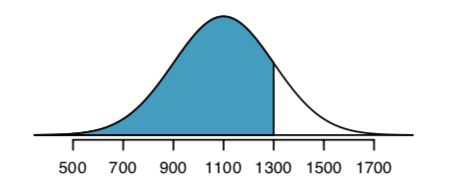
\includegraphics[scale=0.5]{images/tailarea.png}
    \end{center}
    We can specify the cutoff explicitly if we also note the mean and standard deviation:
    
    \hspace{1cm} \texttt{> pnorm(1300, mean = 1100, sd = 200))} \\ \hspace{1cm}\texttt{[1] 0.8413447}
\end{frame}

\begin{frame}{Finding Tail Areas}
    \begin{itemize}
        \item For quizzes and exams, you will be provided with information from \texttt{R}. 
        \item I will do the work in \texttt{R}, but you will need to use a Z-score to pick the correct tail probability from a list.
    \end{itemize}
    For example
    \begin{center}
        \begin{tabular}{l l}
            \hline
            Z-score & Lower Tail Area \\
            \hline
            1 & 0.8413 \\
            1.5 & 0.9332 \\
            \hline
        \end{tabular}
    \end{center}
\end{frame}

\begin{frame}{Finding Tail Areas}
    \begin{itemize}
        \item We will solve all normal distribution problems by first calculating Z-scores.
        \item We do this because it will help us when we move on to Chapter 5.
        \item Therefore all tail area information will be provided in terms of Z-scores (as in the previous slide).
    \end{itemize}
\end{frame}

\begin{frame}{Example: Normal Probability}
    Cumulative SAT scores are well-approximated by a normal model, $N (\mu = 1100, \sigma = 200)$.
    
    \vspace{12pt}Shannon is a randomly selected SAT taker, and nothing is known about her SAT aptitude. What is the probability Shannon scores at least 1190 on her SATs?
\end{frame}

\begin{frame}{Normal Probability}
    This brings up a crucial point:
    \begin{itemize}
        \item The area under a distribution curve is 1. 
        \item This corresponds to the probabilities in a discrete probability distribution summing to 1!
    \end{itemize}
    So when we want to know the probability Shannon scores at least 1190 on her SATs, we are interested in $P(X < 1190)$.
\end{frame}

\begin{frame}{Example: Normal Probability}
    SATs well approximated by $N (\mu = 1100, \sigma = 200)$
    \begin{itemize}
        \item First, we want to draw and label a picture of the normal distribution.
        \item These do not need to be exact to be useful.
        \begin{itemize}
            \item We will see this in a moment when I try to draw on the board.
        \end{itemize}
        \item We are interested in the chance she scores above 1190, so we shade the upper tail.
    \end{itemize}
\end{frame}

\begin{frame}{Example: Normal Probability}
    To find the area of the shaded section
    \begin{itemize}
        \item First calculate the Z-score
        \[
            Z = \frac{x-\mu}{\sigma} = \frac{1190-1100}{200} = 0.45
        \]
        \item Then find the lower tail probability (using a statistical software or other method). 
        \begin{itemize}
            \item The area left of $Z = 0.45$ is $0.6736$.
        \end{itemize}
    \end{itemize}
\end{frame}

\begin{frame}{Example: Normal Probability}
    \begin{center}
        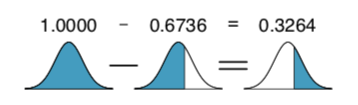
\includegraphics[scale=0.65]{images/normalcomp.png}
    \end{center}
    To find the area above $Z = 0.45$, P$(Z > 0.45)$ we can use the complement,
    \[
        P(Z > 0.45)=1-P(Z<0.45),
    \]
\end{frame}

\begin{frame}{Example: Normal Probability}
    \begin{center}
        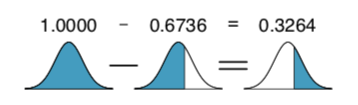
\includegraphics[scale=0.65]{images/normalcomp.png}
    \end{center}
    This is one minus the area of the lower tail:
    \[
        1-0.6737=0.3264
    \]
    So the probability Shannon scores at least 1190 is 32.64\%.
\end{frame}

\begin{frame}{Finding Areas to the Right}
    \begin{itemize}
        \item Software programs usually return the area to the left (left tail) when given a Z-score.
        \item To get the area to the right
        \begin{enumerate}
            \item Find the area to the left.
            \item Subtract this area from one.
        \end{enumerate}
    \end{itemize}
\end{frame}

\begin{frame}{Recommendation}
    \textbf{Draw a picture first; find the Z-score second.}
    \begin{itemize}
        \item Draw and label the normal curve and shade the area of interest.
        \item This helps to 
        \begin{enumerate}
            \item Provide a general estimate of the probability.
            \item Set up your problem correctly.
        \end{enumerate}
        \item \textit{Then} you can identify the appropriate Z-score and probabilities.
    \end{itemize}
\end{frame}

\begin{frame}{Example}
    Edward earned a 1030 on his SAT. What is his percentile?
\end{frame}

\begin{frame}{Example}
    Edward earned a 1030 on his SAT. What is his percentile? Recall that his percentile is the percent of people who score lower than Edward.
    
    \vspace{12pt}First, we want to draw a picture. Recall that cumulative SAT scores are well-approximated by a normal model, $N (\mu = 1100, \sigma = 200)$
\end{frame}

\begin{frame}{Example}
    Identifying the mean $\mu = 1100$, the standard deviation $\sigma = 200$, and the cutoff for the tail area $x = 1030$ makes it easy to compute the Z-score:
    \[
        Z = \frac{x-\mu}{\sigma} = \frac{1030-1100}{200}=-0.35
    \]
    
    \vspace{12pt}Using \texttt{R}, we get a (left) tail area of 0.3632.
    
    \vspace{12pt}So Edward is at the 36th percentile.
\end{frame}

\begin{frame}{Example}
    Use the results of the previous example to compute the proportion of SAT takers who did better than Edward.
\end{frame}

\begin{frame}{Example}
    Use the results of the previous example to compute the proportion of SAT takers who did better than Edward.
    
    \vspace{12pt}Let's revise our picture.
\end{frame}

\begin{frame}{Example}
    We know that 36.32\% of test-takers do worse than Edward. So
    \begin{align*}
        P(\text{better than Edward}) &= 1-P(\text{not better than Edward}) \\
            &= 1-0.3632 \\
            &= 0.6368
    \end{align*}
\end{frame}

\begin{frame}{Percentiles}
    \begin{itemize}
        \item So far, we've talked about finding a percentile based on an observation.
        \item Now we want to think about finding the observation corresponding to a particular percentile.
        \item For example, suppose you want to get into a graduate school whose incoming students usually score above the 80th percentile on the GRE.
        \begin{itemize}
            \item We might be interested in estimating what score corresponds to the 80th percentile.
        \end{itemize}
    \end{itemize}
\end{frame}

\begin{frame}{Example: Percentiles}
    Based on a sample of 100 men, the heights of male adults in the US is nearly normal with mean 70.0” and standard deviation 3.3”. 
    
    \vspace{12pt}Erik’s height is at the 40th percentile. How tall is he?
\end{frame}

\begin{frame}{Example: Percentiles}
    Heights are approximately normal $N(\mu=70, \sigma=3.3)$. Erik is at the 40th percentile.
    
    \vspace{12pt}First, we want to draw our picture.
\end{frame}

\begin{frame}{Example: Percentiles}
    Heights are approximately normal $N(\mu=70, \sigma=3.3)$. Erik is at the 40th percentile.
    
    \vspace{12pt}\begin{itemize}
        \item Before, we knew the Z-score and used it to find the area.
        \item Now, we know the area and must find the Z-score.
    \end{itemize}
    
    Using \texttt{R}, we obtain the corresponding Z-score of $z=-0.25$.
\end{frame}

\begin{frame}{Example: Percentiles}
    Heights are approximately normal $N(\mu=70, \sigma=3.3)$. Erik is at the 40th percentile.
    
    \vspace{12pt}Now we have the corresponding Z-score of $z=-0.25$ and can use the Z-score formula to find Erik's height:
    \[
    -0.25 = z_{Erik} = \frac{x_{Erik}-\mu}{\sigma} = \frac{x_{Erik}-70}{3.3}
    \]
\end{frame}

\begin{frame}{Example: Percentiles}
    With a little algebra, we can solve for $x_{Erik}$:
    \[
    x_{Erik}=-0.25\times3.3 + 70=69.175
    \]
    So Erik is about 5'9.
\end{frame}

\begin{frame}{Example: Percentiles}
    What is the adult male height at the 82nd percentile?
    
    \vspace{12pt}As always, we begin by drawing our picture.
\end{frame}

\begin{frame}{Example: Percentiles}
    What is the adult male height at the 82nd percentile?
    
    \vspace{12pt}We need to find the Z-score at the 82nd percentile
    \begin{itemize}
        \item This will be a positive value and can be found using software as $z = 0.92$. 
    \end{itemize}
\end{frame}

\begin{frame}{Example: Percentiles}
    What is the adult male height at the 82nd percentile?
    
    \vspace{12pt}
    Finally, the height $x$ is found using the Z-score formula with the known mean $\mu=70$, standard deviation $\sigma=3.3$, and Z-score $z = 0.92$:
    \[
        0.92 = z = \frac{x-\mu}{\sigma} = \frac{x-70}{3.3}
    \]
    and so $x=0.92\times3.3 + 70=73.04$
\end{frame}

\begin{frame}{Example: Percentiles}
    What is the adult male height at the 50th percentile?
    
    \vspace{12pt}As always, we begin by drawing our picture.
\end{frame}

\begin{frame}{The 50th Percentile}
    \begin{itemize}
        \item When we talked about measures of center, we noted that the 50th percentile is the median.
        \item Because the normal distribution is \textit{symmetric}, the mean and median will be equal.
        \item This means that for the normal distribution the 50th percentile will always be $\mu$.
    \end{itemize}
\end{frame}

\begin{frame}{Example}
    Adult male heights follow $N(70.0,3.3)$.
    \begin{enumerate}
        \item What is the probability that a randomly selected male adult is at least 6’2 (74 inches)?
        \item What is the probability that a male adult is shorter than 5’9” (69 inches)?
    \end{enumerate}
    
    \vspace{12pt}Let's start by drawing a picture for each.
\end{frame}

\begin{frame}{Example}
    Adult male heights follow $N(70.0,3.3)$. What is the probability that a randomly selected male adult is at least 74 inches?
    
    \vspace{12pt}First, we calculate the Z-score:
    \[
        z_{74}=\frac{74-70}{3.3}=1.21
    \]
    
    Using software, the left tail area is 0.8869, but we want the probability that he is \textit{at least} 74 inches:
    \[
    1-0.8869 =0.1131
    \]
\end{frame}

\begin{frame}{Example}
    Adult male heights follow $N(70.0,3.3)$. What is the probability that a male adult is shorter than 69 inches?
    
    \vspace{12pt}First, we calculate the Z-score:
    \[
        z_{74}=\frac{69-70}{3.3}=-0.30
    \]
    
    Using software, the left tail area is 0.3821. We want the probability that he is shorter than 69 inches, so this is the value we want.
\end{frame}

\begin{frame}{Interval Probabilities}
    What is the probability that a random adult male is \textit{between} 69 and 74 inches?
    
    \vspace{12pt}First, let's draw a picture. We will compare this picture to the two from the previous example.
\end{frame}

\begin{frame}{Interval Probabilities}
    What is the probability that a random adult male is \textit{between} 69 and 74 inches?
    
    \vspace{12pt}The total area under the curve is 1. We've already calculated
    \[
        P(\text{height} > 74)
    \]
    and 
    \[
        P(\text{height} < 69).
    \]
    We want to calculate
    \[
        P( 69 < \text{height} < 74).
    \]
\end{frame}

\begin{frame}{Interval Probabilities}
    We can use our drawings to visualize what we want to calculate:
    \begin{center}
        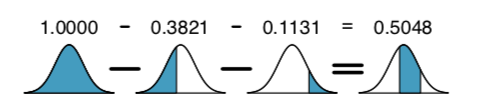
\includegraphics[scale=0.6]{images/intprob.png}
    \end{center}
    So the probability of being between 69 and 74 inches tall is about 50.5\%.
\end{frame}

\begin{frame}{Example}
    SAT scores follow $N(1100,200)$. What percent of SAT takers get between 1100 and 1400?
    
    \vspace{12pt}We'll start with a picture.
\end{frame}

\begin{frame}{Example}
    We want the area between the two tails, so we are going to calculate the tail areas and then subtract them from one.
    
    \vspace{12pt}We'll start with $P(\text{score}<1100)$. SAT scores follow $N(1100,200)$.
    \begin{itemize}
        \item Notice that this is the mean.
        \item We know that for the normal distribution, the mean and median are the same.
        \item So we know that this is the 50th percentile.
    \end{itemize}
    So, $P(\text{score}<1100)=0.5$
\end{frame}

\begin{frame}{Example}
    We want the area between the two tails, so we are going to calculate the tail areas and then subtract them from one.
    
    \vspace{12pt}Now we'll examine $P(\text{score}>1400)$. SAT scores follow $N(1100,200)$. The Z-score is
    \[
        z = \frac{1400-1100}{200} = 1.5
    \]
    Using \texttt{R}, the corresponding percentile is 0.9332, but we want the upper tail:
    \[
        1-0.9332=0.0668
    \]
\end{frame}

\begin{frame}{Example}
    Finally, we will subtract both of these tail probabilities from one to get the area between the two percentiles:
    \[
    1-0.5-0.0668=0.4332
    \]
    So 43.32\% of SAT takers get scores between 1100 and 1400.
\end{frame}

\begin{frame}{The 68-95-99.7 Rule}
    The 68-95-99.7 Rule is a good general rule for thinking about the normal distribution.
    
    \begin{itemize}
        \item 68\% of the observations will fall within 1 standard deviation of the mean
        \item 95\% of the observations will fall within 2 standard deviations of the mean
        \item 99.7\% of the observations will fall within 3 standard deviations of the mean
    \end{itemize}
    This can be useful when trying to make a quick Z-score estimate without access to software.
\end{frame}

\begin{frame}{The 68-95-99.7 Rule}
    \begin{center}
        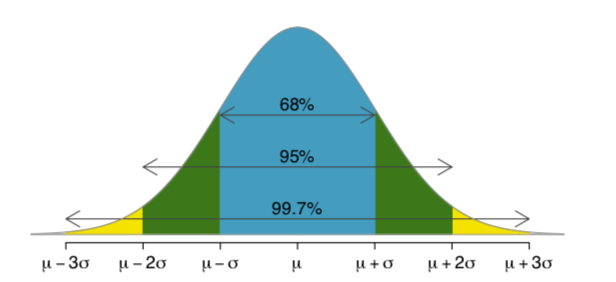
\includegraphics[scale=0.5]{images/rule68_95_997.png}
    \end{center}
\end{frame}

\begin{frame}{Outliers}
    We can also use Z-score and the 68-95-99.7 Rule to look for outliers.
    \begin{itemize}
        \item We expect 95\% of the observations to fall within 2 standard deviations, so observations outside of this are \textit{unusual}.
        \item We expect 99.7\% of the observations to fall within 3 standard deviations, so observations outside of this are very unusual or \textit{outliers}.
    \end{itemize}
    We can certainly have observations outside of 3 or 4 standard deviations from the mean, but the probability of being further than 4 standard deviations from the mean is about 1-in-15,000.
\end{frame}

\begin{frame}{The 68-95-99.7 Rule}
    \begin{center}
        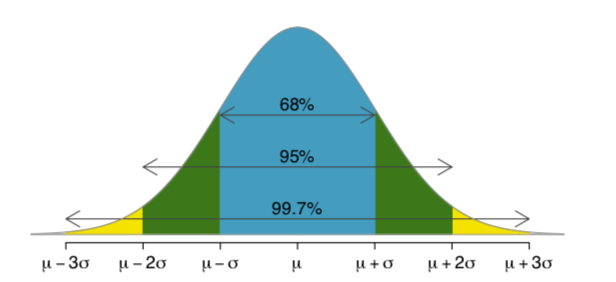
\includegraphics[scale=0.5]{images/rule68_95_997.png}
    \end{center}
    We will confirm these probabilities in Lab 5.
\end{frame}